\documentclass[border=6pt]{standalone}
\usepackage{amsmath}
\usepackage{tikz}
\usetikzlibrary{arrows.meta}
\begin{document}
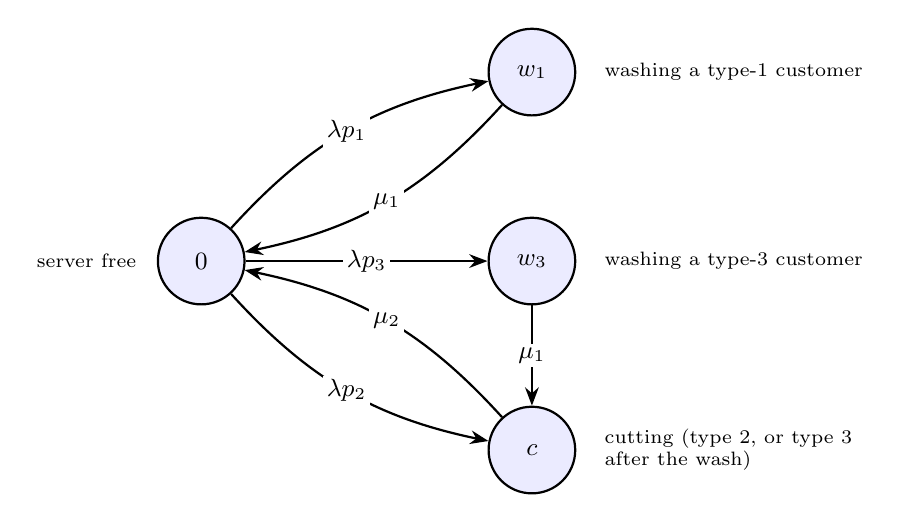
\begin{tikzpicture}[>=Stealth,font=\small,
 s/.style={draw,thick,circle,minimum size=1.1cm,inner sep=0pt,fill=blue!8},
 e/.style={->,thick},
 lab/.style={font=\small,fill=white,inner sep=1.5pt},
 every loop/.style={->,thick,looseness=6}]
\node[s] (0) at (0,0) {$0$};
\node[s] (w1) at (4.2,2.4) {$w_1$};
\node[s] (w3) at (4.2,0) {$w_3$};
\node[s] (c) at (4.2,-2.4) {$c$};
\draw[e] (0) to[bend left=18] node[lab]{$\lambda p_1$} (w1);
\draw[e] (w1) to[bend left=18] node[lab]{$\mu_1$} (0);
\draw[e] (0) -- node[lab]{$\lambda p_3$} (w3);
\draw[e] (w3) -- node[lab]{$\mu_1$} (c);
\draw[e] (0) to[bend right=18] node[lab]{$\lambda p_2$} (c);
\draw[e] (c) to[bend right=18] node[lab]{$\mu_2$} (0);
\node[font=\scriptsize,align=left,anchor=west] at (5.0,2.4) {washing a type-1 customer};
\node[font=\scriptsize,align=left,anchor=west] at (5.0,0) {washing a type-3 customer};
\node[font=\scriptsize,align=left,anchor=west] at (5.0,-2.4) {cutting (type 2, or type 3\\after the wash)};
\node[font=\scriptsize,anchor=east] at (-0.7,0) {server free};
\end{tikzpicture}
\end{document}
